\chapter{Identificación de subsistemas}
\label{ch:subsistemas}

En base a los requisitos elaborados y al plan de diseño y arquitectura sopesados para el sistema se han identificado los siguientes subsistemas internos a los dos subsistemas mayores del sistema: la aplicación móvil y la \acrshort{api}. Así como la comunicación entre dichos subsistemas y sus subsistemas internos.

\section{Aplicación móvil}
\label{sec:subsistema_app}

De cara a seguir las principales indicaciones en el desarrollo de sistemas Android, se ha decidido utilizar la arquitectura \acrshort{mvvm}\cite{mvvm2021} y, por consiguiente, su misma especificación de subsistemas.

\subsection{Actividades}

Las actividades conforman los mayores componentes de una aplicación Android pues gestionan las pantallas mostradas al usuario y toda lógica de estados y funcionalidad ofrecida por dicha pantalla. Con la aplicación de la arquitectura \acrshort{mvvm} estos componentes se componen a su vez de dos subsistemas interrelacionados.

\subsubsection{Modelos de vista}

Los modelos de vista suponen la novedad introducida por la arquitectura a utilizar y son módulos encargados de extraer la lógica de datos de las actividades para separarlos de la vista. El modelo de vista contiene la información que se mostrará en pantalla o que sea necesaria para la ejecución de la aplicación, y de la misma forma está a cargo de la obtención de esta, gestionando la comunicación con subsistemas inferiores.

\subsubsection{Vistas}

Las vistas son el sistema en control de la lógica de dibujado, animación y manejo de los elementos de la interfaz de usuario. Recuperan la información contenida en sus modelos de vista y la muestran por pantalla. Están compuestas por archivos de diseño de la interfaz y por archivos de código para las gestiones más complejas de la misma.

\subsection{Modelo}

La representación de las entidades de datos a manejar en la aplicación. Son las entidades que se usarán en la comunicación entre subsistemas y carecerán de más responsabilidades que la de manejarse a sí mismas.

\subsection{Repositorios}

Capa de comunicación entre las actividades y los servicios o bases de datos. Tendrán la responsabilidad de comunicarse con los módulos necesarios para obtener los datos solicitados por las actividades y de la transformación de los mismos en los modelos que serán usados en la aplicación. También gestionarán las peticiones en la dirección contraria, solicitando a los servicios acciones sobre entidades proporcionadas por las actividades.

\subsection{Servicios}

Los servicios son la capa más profunda de la aplicación y son los encargados de la comunicación directa con las bases de datos o interfaces web. En el primer planteamiento de la aplicación no se ha estimado la presencia de una base de datos local por lo que los únicos servicios serán todos web. Sin embargo, dentro de los servicios web podremos distinguir dos tipos: unos enfocados en la comunicación \acrshort{http} y otros en la comunicación por medio del protocolo WebSocket.

\section{API}

Para la \acrshort{api} se ha distinguido un total de tres subsistemas mayores relacionados mutuamente en un esquema triangular que invalida el planteamiento de arquitecturas por capas.

\subsection{Bases de datos}

El subsistema a cargo de gestionar la persistencia y recuperación de datos estará compuesto por dos partes interrelacionadas:

\subsubsection{Modelo}

Los modelos serán la representación de las entidades almacenadas en la base de datos y que serán recuperadas por los dos subsistemas superiores. Carecen de toda lógica que no implique su autogestión y serán siempre modificados, creados, leídos o eliminados por los servicios.

\subsubsection{Servicios}

Sistema de gestión del Modelo de la base de datos. Módulos encargados de manejar las consultas y operaciones de la base de datos con toda la lógica necesaria para aseverar la consistencia y restricciones necesarias en los datos. Son el único sistema con capacidad de manejo sobre el Modelo.

\subsection{Manejador HTTP REST}

Módulo a cargo de recibir y gestionar las peticiones \acrshort{http} para la \acrshort{api} \acrshort{rest}. Contiene la lógica de las operaciones a realizar para cumplir la petición, de todas las comprobaciones necesarias y del manejo de error de las mismas en caso de que surjan errores o sean incorrectas. Realizan las operaciones concernientes a los datos por medio de los servicios, quedando en la lógica de este manejador únicamente la gestión del flujo de operaciones.

\subsection{Manejador WebSocket}

Similar al manejador \acrshort{http} \acrshort{rest} pero con la diferencia de que este subsistema escucha los mensajes recibidos por medio de la interfaz WebSocket. Contiene la lógica para gestionar los eventos notificados a través del mismo y para responder a estos de vuelta o por retransmisión a través del socket. Como el otro manejador, todas sus operaciones son únicamente llamadas sucesivas a los servicios necesarios.

\section{Comunicación entre subsistemas}

Para satisfacer el funcionamiento total de los subsistemas de la aplicación se ha definido la siguiente comunicación que garantice la integridad de las arquitecturas.

\subsection{Subsistemas internos de la aplicación móvil}

La comunicación de los subsistemas de la aplicación seguirá también la arquitectura \acrshort{mvvm} y como esta define la comunicación entre sus subsistemas. El diagrama \ref{fig:sub-app} que lo representa está basado en el mismo diagrama del artículo de referencia de Google\cite{mvvm2021}.

Dentro de la aplicación la comunicación entre subsistemas será vertical y unidireccional. Las vistas solo serán accedidas por la propia interacción del usuario y a su vez serán las únicas que se comuniquen con sus modelos de vista. Esto se hará por medio de llamadas para la ejecución de operaciones o mediante el patrón observador sobre los datos (usando objetos LiveData\cite{liveData2021} de Android) gestionados y almacenados por el modelo de vista.

El modelo de vista por su parte estará a cargo de proveer cualquier necesidad de la vista y para toda la lógica que implique una comunicación externa o la persistencia o recuperación de datos se servirá de los repositorios. Los repositorios llamarán a los servicios necesarios para que tramiten la petición y recuperar la información necesaria o llevar a cabo la operación encomendada desde el modelo de vista contactando con la API.

\begin{figure}[H]
    \centering
    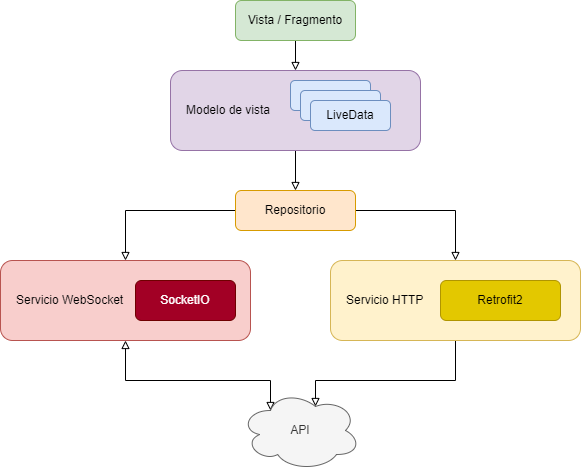
\includegraphics[width=0.6\textwidth]{Analisis/ComunicacionSubsistemasApp.drawio.png}
    \caption{Arquitectura y comunicación de la aplicación móvil}
    \label{fig:sub-app}
\end{figure}

\subsection{Subsistemas internos de la API}

La \acrshort{api} puede recibir comunicaciones por dos vías diferentes. Por peticiones \acrshort{http} a través de su \acrshort{api} \acrshort{rest} y por medio del socket a través de su interfaz WebSocket. A su vez, peticiones \acrshort{http} pueden requerir el envío de eventos a través del socket, por lo que es necesario que exista comunicación entre estos dos subsistemas. Dicha comunicación será llevada a cabo por medio de la referencia recíproca al manejador raíz de ambos subsistemas, de forma que se puedan realizar llamadas mutuas. A su vez, ambos subsistemas requieren la comunicación con la base de datos que realizarán a partir de los servicios.

\begin{figure}[H]
    \centering
    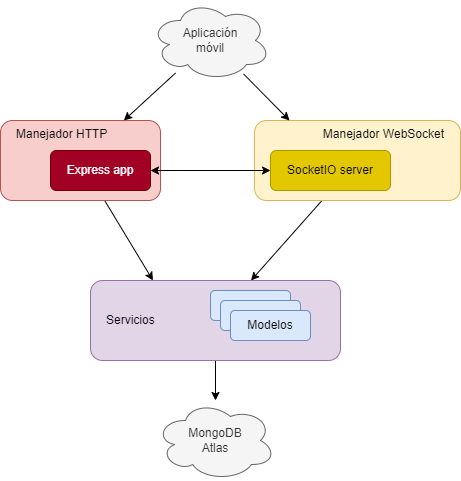
\includegraphics[width=0.4\textwidth]{Analisis/ComunicacionSubsistemasAPI.drawio.png}
    \caption{Arquitectura y comunicación de la API}
    \label{fig:sub-api}
\end{figure}

\subsection{Subsistemas API y aplicación móvil}

Finalmente, de cara a que el sistema funcione se ha definido también la comunicación entre los dos mayores componentes. La comunicación entre la aplicación y la \acrshort{api} tendrá dos vías distintas. Por un lado estarán las peticiones \acrshort{http} realizadas a través de la librería \textbf{Retrofit 2} (\fref{lib:app:retrofit2}) que la \acrshort{api} gestionará y responderá a través de los \gls{endpoint} servidos por medio de su \acrshort{api} \acrshort{rest} construída sobre el framework Express (\fref{lib:api:express}). Y por otro lado, al iniciar la aplicación se establecerá un canal \acrshort{tcp} entre la aplicación y la \acrshort{api} utilizando Socket.IO (\fref{lib:api:socket_io}) en ambos extremos de esta comunicación.

\begin{figure}[H]
    \centering
    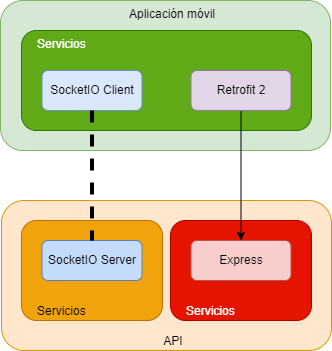
\includegraphics[width=0.3\textwidth]{Analisis/ComunicacionSistemas.drawio.png}
    \caption{Comunicación entre la aplicación y la API}
    \label{fig:sub-comunicacion}
\end{figure}